\documentclass[handout]{beamer} % Use the beamer class for presentations, 'handout' option to suppress \pause

\input{Lecture-Slides/preamble.txt}

% 1) Define the CSV data for the two distributions using filecontents
\begin{filecontents*}{dist1.csv}
x,y
1,0.05
2,0.10
3,0.20
4,0.30
5,0.20
6,0.10
7,0.05
\end{filecontents*}

\begin{filecontents*}{dist2.csv}
x,y
1,0.01
2,0.05
3,0.25
4,0.5
5,0.25
6,0.05
7,0.01
\end{filecontents*}


% Define the transition slide command
\newcommand{\transitionslide}[1]{
    \begin{frame}[plain]
          \addtocounter{framenumber}{-1}
        \centering
        \vspace{1cm}
        \Huge
        \textcolor{moonstoneblue!150}{\textbf{#1}}
    \end{frame}
}


\title{Introduction to Statistical Methods in Political Science}
\subtitle{Lecture 2: Summarizing Data I - Descriptive Statistics}
\author{Ignacio Urbina}
\date{}

\begin{document}

\frame{\titlepage}

%%%%%%%%%%%%%%%%%%%%%%%%%%%%%%%%%%%%%%%%
\section{Descriptive Statistics}
\transitionslide{Descriptive Statistics}

% Slide 1: Keeping the goal in sight
\begin{frame}
\frametitle{Keeping the Goal in Sight}
\begin{itemize}
\item Recap: Inferential statistics $\rightarrow$ Learning about the properties and characteristics of a population using samples.
\item Recall that we call a `statistic' any quantitative value that is a function of our sample data and, through a specific function, maps them into a single measurement meant to represent a feature of the data.
\end{itemize}
\end{frame}

% Slide 2: Descriptive Statistics
\begin{frame}
\frametitle{Descriptive Statistics}
\begin{itemize}
\item Before making inferences about the population, it is essential to learn how to effectively describe the properties and characteristics of the data we collected in our sample.
\item We call this process “descriptive statistics” and use different measures (statistics) to describe our data.
\item We have three types of descriptive statistics: univariate, bivariate, and multivariate.
\end{itemize}
\end{frame}

% Slide 3: Distribution of a Variable
\begin{frame}
\frametitle{Distribution of a Variable}
\begin{itemize}
\item At a fundamental level, when doing descriptive statistics, our goal is to provide a summarized description of the distribution of our data.
\item \emph{Def.} \textbf{Distribution of a variable}. The distribution of a variable is a function (often represented in a graph) that shows the possible values of a variable and how often they occur.
\end{itemize}
\end{frame}

\begin{frame}
\frametitle{Distribution of a Continuous Variable}

\begin{center}
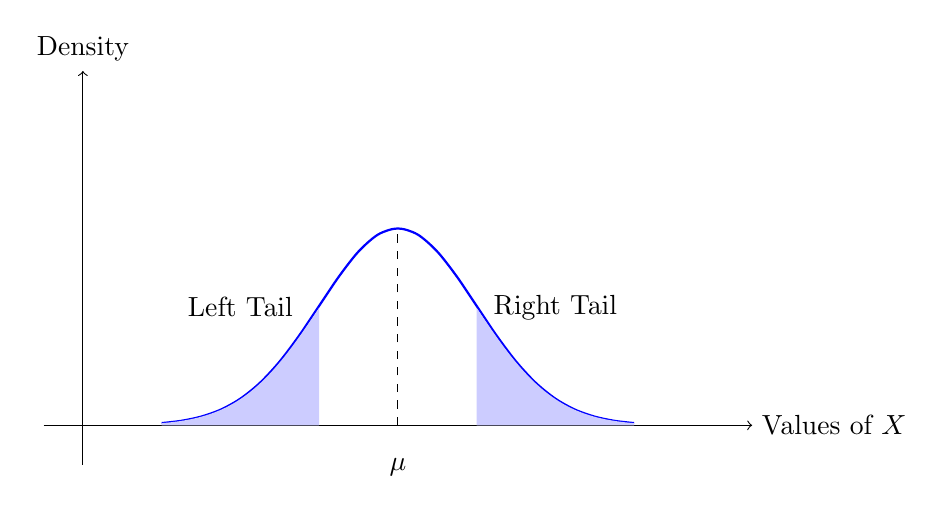
\begin{tikzpicture}
    % Axes
    \draw[->] (-0.5,0) -- (8.5,0) node[right] {Values of $X$};
    \draw[->] (0,-0.5) -- (0,4.5) node[above] {Density};

    % Distribution curve
    \draw[thick, domain=1:7, smooth, variable=\x, blue] plot ({\x},{2.5*exp(-0.5*(\x-4)^2)});

    % Labels
    \node at (4,-0.3) [below] {$\mu$};
    \draw[dashed] (4,0) -- (4,2.5);
    \node at (2,1.5) {Left Tail};
    \node at (6,1.5) {Right Tail};

    % Shading for left tail
    \fill[blue!20] (1,0) -- plot[domain=1:3, smooth] ({\x},{2.5*exp(-0.5*(\x-4)^2)*0.984}) -- (3,0) -- cycle;

    % Shading for right tail
    \fill[blue!20] (5,0) -- plot[domain=5:7, smooth] ({\x},{2.5*exp(-0.5*(\x-4)^2)*0.984}) -- (7,0) -- cycle;
\end{tikzpicture}
\end{center}

\end{frame}

\begin{frame}
\frametitle{Distribution of Categorical Ordinal Data}

\begin{figure}
\centering
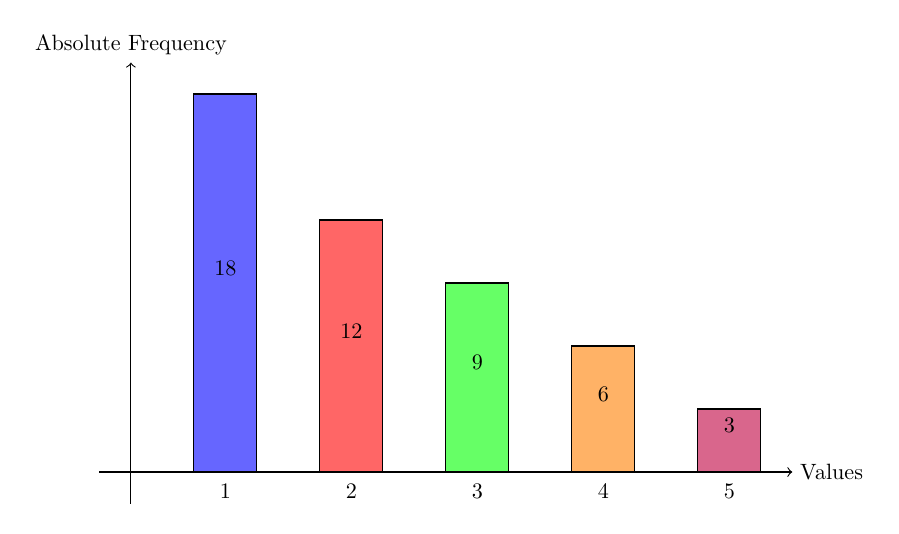
\begin{tikzpicture}[scale=0.8, transform shape]

    % Axes
    \draw[->] (-0.5,0) -- (10.5,0) node[right] {Values};
    \draw[->] (0,-0.5) -- (0,6.5) node[above] {Absolute Frequency};

    % Bars for categories
    \draw[fill=blue!60] (1,0) rectangle (2,6) node[midway, above] {18};
    \draw[fill=red!60]  (3,0) rectangle (4,4) node[midway, above] {12};
    \draw[fill=green!60] (5,0) rectangle (6,3) node[midway, above] {9};
    \draw[fill=orange!60] (7,0) rectangle (8,2) node[midway, above] {6};
    \draw[fill=purple!60] (9,0) rectangle (10,1) node[midway, above] {3};

    % Value labels
    \node at (1.5,-0.3) {1};
    \node at (3.5,-0.3) {2};
    \node at (5.5,-0.3) {3};
    \node at (7.5,-0.3) {4};
    \node at (9.5,-0.3) {5};

\end{tikzpicture}
\caption{Categorical Ordinal Distribution}
\end{figure}

\end{frame}



% Slide 4: Summarizing Data
\begin{frame}
\frametitle{Summarizing Data}
\begin{itemize}
\item Datasets often include hundreds, thousands, and, on some occasions, millions of observations. While looking at the dataset is always instructive, it is impossible to make sense of it just by doing so.
\item Hence, we need to summarize our data. By this, we mean \textbf{aggregating} —or putting all the data together—into a few pieces of information that are far easier to read and interpret.
\end{itemize}
\end{frame}

% Slide 5: How to Describe Data
\begin{frame}
\frametitle{How to Describe Data}
\begin{itemize}
\item When we summarize data we, again, seek to provide a summarized description of the distribution of a variable.
\item In \textbf{univariate descriptive statistics}, we will describe the distribution of a variable using three approaches:
\begin{itemize}
    \item Measures of Central Tendency
    \item Measures of Dispersion Around the Center
    \item Shape of the Distribution
\end{itemize}
\end{itemize}
\end{frame}

\section{Measures of Central Tendency}

% Slide 6: Measures of Central Tendency
\begin{frame}
\frametitle{Measures of Central Tendency}
\begin{itemize}
\item We are often interested in describing a distribution by providing one value representing its center.  \pause % <-----|
\item By ``center," we mean a numeric value that balances the distance between all the other points in the distribution in some specific way. \pause % <-----|
\item Depending on a variable's specific type of distribution and the type of variable (categorical or numerical), we will use the \textbf{average}, \textbf{median}, or \textbf{mode} to best represent the center of the distribution. 
\end{itemize}
\end{frame}

% Slide 7: Central Tendency: the Average (Arithmetic Mean)
\begin{frame}
\frametitle{Central Tendency: the Average (Arithmetic Mean)}
The following is the function (formula) for the \textbf{average} or \textbf{sample mean}:
\begin{equation*}
\bar{X} = \frac{\sum_{i=1}^{N} x_i}{N} = \frac{x_1 + x_2 + \cdots + x_{N-1} + x_{N}}{N}
\end{equation*}
Where:
\begin{itemize}
    \item $i$ represents an arbitrary index we use to label our observations in our sample
    \item The total number of observations is denoted by the letter $N$, and we call it ``sample size." (also $N$ rows in our dataset)
\end{itemize}
\end{frame}

% Slide 8: The Average: Some Notes
\begin{frame}
\frametitle{The Average: Some Notes}
\begin{itemize}
\item Why is the average useful? The average is useful because it provides a single measure summarising the entire dataset with just one value. 
\begin{itemize}
    \item This simplifies our understanding of and ability to work with data. Despite being affected by outliers, the average is still important in various statistical analyses.
\end{itemize}
\item \emph{Caveat}: the average does not necessarily equal the value most likely to be randomly drawn from the data.
\end{itemize}
\end{frame}

% Slide 9: On Outliers or Extreme Values
\begin{frame}
\frametitle{On Outliers or Extreme Values}
\begin{itemize}
\item Sometimes the data will have extreme values, which are values that according to the pre-established criteria (we will review this in time) can be deemed as extremely far from the center of the distribution, such that these values are very unlikely.
\item In small samples, these outliers can disturb the usefulness of the mean as a description of central tendency, such that the information they provide is of lesser qualitative significance.
\end{itemize}
\end{frame}

% Slide 10: Example of Influence of Outliers
\begin{frame}
\frametitle{Example of Influence of Outliers}
\begin{itemize}
\item Imagine we have a sample size of $N_{\text{Sample 1}}=10$. We have measured a random sample of people’s yearly income. Assume we find $\bar{X}_{\text{Sample 1}} = 40,000$. 
\item Now consider another sample, this time of size $N_{\text{Sample 2}} = 1,000$. Assume we find that $\bar{X}_{\text{Sample 2}} = 42,500$.
\item Assume in each sample, we forgot to include an additional data point: $X_{N+1} = 150,000$. How does the mean change in each case?
\end{itemize}
\end{frame}

% Slide 11: Central Tendency: the Median
\begin{frame}
\frametitle{Central Tendency: the Median}
\begin{itemize}
\item When numerical data have a natural ordering, we can also use an alternative measure of central tendency: the \textbf{median}. \pause % <-----|
\item The median is the \emph{value of the distribution that lies in the middle} such that 50\% of the values are to the left and 50\% to the right. \pause % <-----|
\item In other words, with the median, our notion of distance from the ``center" is more concerned with rank order than numeric absolute distance.
\end{itemize}
\end{frame}

% Slide 12: Central Tendency: the Median
\begin{frame}
\frametitle{Central Tendency: the Median}

Here’s the general formula for the median depending on whether $N$ is odd or even:
\begin{equation*}
median(X) = 
\begin{cases} 
X_{\{\frac{N+1}{2}\}} & \text{if $N$ is odd} \\
\frac{1}{2}(X_{\{\frac{N}{2}\}} + X_{\{\frac{N}{2} + 1\}}) & \text{if $N$ is even}
\end{cases}
\end{equation*}


\begin{itemize}
\item In the presence of outliers, the median can be a more resilient measure of central tendency than the mean, especially in small samples.
\item Why? Because the median only considers the rank order of the values of the distribution, therefore, it is robust against outliers.
\end{itemize}

\end{frame}

% Slide 13: Central Tendency: The Mode
\begin{frame}
\frametitle{Central Tendency: The Mode}
\begin{itemize}
\item Another central tendency summary statistic is the mode, which is particularly useful for categorical values.
\item \emph{Def.} \textbf{Mode}: The mode is the most frequent value of the distribution.
\item Because of this definition, the mode is also considered the most likely value of the distribution.
\item Yet, in practice, the mode is only useful for categorical values (It is important to think why this is the case).
\end{itemize}
\end{frame}

% Slide 14: Some Notes: The Mode
\begin{frame}
\frametitle{Some Notes: The Mode}
\begin{itemize}
\item Note that the mode is also a robust statistic in that it is resilient against outliers.
\item When a distribution has only one mode, we call it “unimodal;” when it has two, we call it “bimodal.”
\item While we might be tempted to always prefer the mode as a measure of central tendency for categorical variables, in practice, we should always look at all the \emph{appropriate} measures of central tendency jointly when asking about the central tendency of a distribution.
\end{itemize}
\end{frame}


\section{Distributions: Absolute, Relative, and Cumulative Frequency}
\transitionslide{Distributions: Absolute, Relative, and Cumulative Frequency}

% Slide 15: More on Distributions: Absolute and Relative Frequency
\begin{frame}
\frametitle{More on Distributions: Absolute and Relative Frequency}
\begin{itemize}
\item Sometimes we want to ask how likely is one specific value of a variable relative to others. This is particularly relevant for variables that take on integer values (nominal and ordinal categorical variables).
\item \emph{Def.} \textbf{Absolute Frequency} of the value of a variable. The absolute frequency of a value is the count of the number of times that value occurs in the data set.
\item \emph{Def.} \textbf{Relative frequency} of the value of a variable. The relative frequency of a value, $f_i$, is the proportion of the total number of data points that that value, $x_i$, represents. 
\begin{itemize}
    \item  It is calculated by dividing the absolute frequency of the value by the total number of data points.
\end{itemize}

\end{itemize}
\end{frame}


% Slide 16: Pew’s American Trends Panel (ATP)
\begin{frame}{Pew Research Center's American Trends Panel (ATP)}
\begin{itemize}
    \item \textbf{Design and Sampling:} Multimode, probability-based panel with roughly 10,000 U.S. adults, selected randomly to ensure national representativeness.
    \item \textbf{Recruitment Method:} Initially recruited via random digit dialing (2014-2017), switched to address-based sampling (ABS) from the U.S. Postal Service's CDS file (2018-present).
    \item \textbf{Survey Modes:} Online surveys (computer, tablet, smartphone) and phone interviews with live interviewers, starting in 2024 to include phone survey options.
    \item \textbf{Weighting:} Multistep process to adjust for sampling stages and nonresponse, aligning survey samples with population benchmarks.
\end{itemize}
\end{frame}


% Slide 17: Example of a categorical ordinal surveyed in ATP Wave 116
\begin{frame}
\frametitle{Example of a categorical ordinal surveyed in ATP Wave 116}
\begin{itemize}
\item In ATP Wave 116, one of the questions posed to the participants was:
``\emph{How confident are you that votes cast by absentee or mail-in ballot across the United States will be counted as voters intend in the elections this November?}"
\item The responses (excluding ``No answer") are categorized into several confidence levels, allowing respondents to express their perceptions.
\end{itemize}

{\small \centering
\begin{tabular}{|l|c|}
\hline
Confidence & Absolute Frequency \\
\hline
Not at all confident & 407 \\
Not too confident & 611 \\
Somewhat confident & 967 \\
Very confident & 534 \\
\hline
\end{tabular}
\par}

\end{frame}

% Slide 18: Example of a categorical ordinal surveyed in ATP Wave 116
\begin{frame}
\frametitle{Example of a categorical ordinal surveyed in ATP Wave 116}
\begin{itemize}
\item Using the absolute frequency of responses compute the relative frequencies.
\item $N=2519$
\end{itemize}
\medskip

{\small \centering
\begin{tabular}{|l|c|c|}
\hline
Confidence & Absolute Frequency & Relative Freq. ($f_i$) \\
\hline
Not at all confident & 407 &  \\
Not too confident & 611 &  \\
Somewhat confident & 967 &  \\
Very confident & 534 &  \\
\hline
\end{tabular}
\par}

\end{frame}


% Slide 20: Example of a categorical ordinal surveyed in ATP Wave 116
\begin{frame}
\frametitle{Example of a categorical ordinal surveyed in ATP Wave 116}
\begin{itemize}
\item Using the relative frequency of responses, compute the cumulative frequencies.
\end{itemize}

{\small \centering
\begin{tabular}{|l|c|c|}
\hline
Confidence & Absolute Frequency & Relative Freq. ($f_i$) \\
\hline
Not at all confident & 407 & 0.162 \\
Not too confident & 611 & 0.243 \\
Somewhat confident & 967 & 0.384 \\
Very confident & 534 & 0.212 \\
\hline
\end{tabular}
\par}

\end{frame}
% Sample size: 2544

% Slide 19: More on Distributions: Cumulative Frequency
\begin{frame}
\frametitle{More on Distributions: Cumulative Frequency}
\begin{itemize}
\item When variables have a specific ordering relationship (either increasing/decreasing in magnitude or qualitative intensity), we can compute the cumulative distribution of the variable.
\item \emph{Def.} \textbf{Cumulative frequency} of the value of a variable. The cumulative frequency is the running total of the frequencies.
\item \emph{Def.} \textbf{Cumulative relative frequency} of the value of a variable ($F_i$). The cumulative frequency is the running total of the relative frequencies.
\begin{itemize}
    \item In other words, the cumulative relative frequency tells the sum of each proportion or percentage including and leading up to each data value
\end{itemize}
\end{itemize}
\end{frame}

% Slide 20: Example of a categorical ordinal surveyed in ATP Wave 116
\begin{frame}
\frametitle{Example of a categorical ordinal surveyed in ATP Wave 116}
\begin{itemize}
\item Using the relative frequency of responses, compute the cumulative relative frequencies.
\end{itemize}

\medskip

{\small \centering
\begin{tabular}{|l|c|c|c|}
\hline
& \multicolumn{3}{c|}{Type of Frequency} \\ 
\cline{2-4}
Confidence & Absolute & Relative ($f_i$) & Cumulative ($F_i$)  \\
\hline
Not at all confident & 407 & 0.162 & 0.16 \\
Not too confident & 611 & 0.243 & 0.40 \\
Somewhat confident & 967 & 0.384 & 0.79 \\
Very confident & 534 & 0.212 & 1.00 \\
\hline
\end{tabular}
\par}

\end{frame}

\begin{frame}{Simulation of 1,000 Throws of Four Coins}
    \textbf{Introduction:} In this experiment, we simulate 1,000 independent throws of four fair coins. 
    Each throw results in a certain number of heads (from 0 to 4). We analyze the distribution of the 
    absolute and relative frequencies of these outcomes.
    
    \vspace{1em}
    
    \textbf{Steps of the Experiment:}
    \begin{itemize}
        \item Each throw consists of flipping 4 independent coins.
        \item We record the number of heads obtained in each throw.
        \item The results are summarized in terms of:
        \begin{itemize}
            \item Absolute frequencies.
            \item Cumulative absolute frequencies.
            \item Relative frequencies.
            \item Cumulative relative frequencies.
        \end{itemize}
    \end{itemize}
\end{frame}

\begin{frame}{Simulation of 1,000 Throws of Four Coins}
    \textbf{Results:} 
    
    \vspace{1em}
    
{\small \centering
\begin{tabular}{|p{0.11\textwidth}|p{0.15\textwidth}|p{0.15\textwidth}|
                    p{0.15\textwidth}|p{0.15\textwidth}|}
    \hline
    \# Heads & Absolute Frequency & Cumulative Frequency & Relative Frequency & Cumulative Relative Frequency \\
    \hline
    0 & 75 & 75 & 0.075 & 0.075 \\
    1 & 266 & 341 & 0.266 & 0.341 \\
    2 & 358 & 699 & 0.358 & 0.699 \\
    3 & 247 & 946 & 0.247 & 0.946 \\
    4 & 54 & 1000 & 0.054 & 1.0 \\
    \hline
\end{tabular}
\par}

\end{frame}


\begin{frame}{Relative and Cumulative Frequencies of the Total Number of Heads When Throwing Four Coins}
\vspace{1em}
\hspace{-2.5em}
\begin{minipage}{0.49\textwidth}
    \centering
    \textbf{Relative Frequencies}
    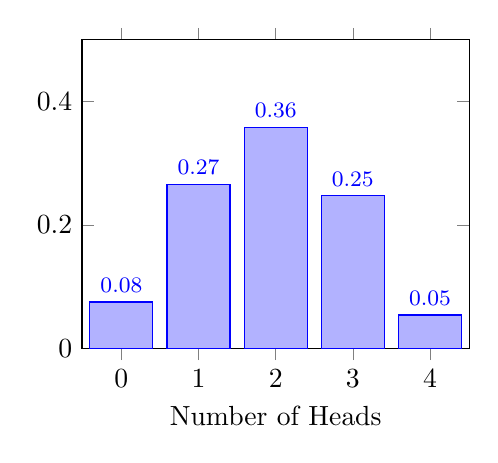
\begin{tikzpicture}
        \begin{axis}[
            ybar,
            bar width=0.8cm,
            symbolic x coords={0, 1, 2, 3, 4},
            xtick=data,
            ymin=0, ymax=0.5,
            xlabel={Number of Heads},
            yticklabel=\pgfmathprintnumber{\tick}, % Fix for scientific notation
            yticklabel style={
                /pgf/number format/fixed, % Forces normal decimal format
                /pgf/number format/precision=3 % Limits decimal places to 3
            },
            scaled ticks=false, % Prevents scientific notation
            nodes near coords,
            every node near coord/.append style={/pgf/number format/fixed,
                font=\footnotesize},
            width=6.5cm, height=5.5cm,
            enlarge x limits={abs=0.5cm},
        ]
        \addplot coordinates {(0,0.075) (1,0.266) (2,0.358) (3,0.247) (4,0.054)};
        \end{axis}
    \end{tikzpicture}
\end{minipage}
\hfill
\begin{minipage}{0.49\textwidth}
    \centering
    \textbf{Cumulative Relative Freq.}
    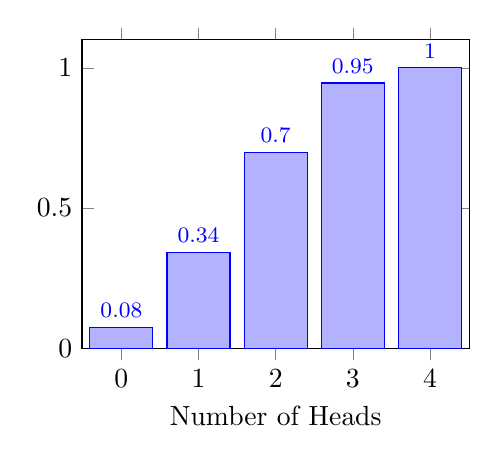
\begin{tikzpicture}
        \begin{axis}[
            ybar,
            bar width=0.8cm,
            symbolic x coords={0, 1, 2, 3, 4},
            xtick=data,
            ymin=0, ymax=1.1,
            xlabel={Number of Heads},
            yticklabel=\pgfmathprintnumber{\tick}, % Fix for scientific notation
            yticklabel style={
                /pgf/number format/fixed, % Forces normal decimal format
                /pgf/number format/precision=3 % Limits decimal places to 3
            },
            scaled ticks=false, % Prevents scientific notation
            nodes near coords,
            every node near coord/.append style={/pgf/number format/fixed,
                font=\footnotesize},
            width=6.5cm, height=5.5cm,
            enlarge x limits={abs=0.5cm},
        ]
        \addplot coordinates {(0,0.075) (1,0.341) (2,0.699) (3,0.946) (4,1.0)};
        \end{axis}
    \end{tikzpicture}
\end{minipage}
\end{frame}



\section{More on the Mean}

% Slide 21: The Weighted Mean
\begin{frame}
\frametitle{The Weighted Mean}
\begin{itemize}
    \item Sometimes, values in a distribution carry different importance because their relative frequencies vary.
    \item Therefore, when computing the mean, we want to account for these different relative frequencies. To do so, we use the weighted mean.
    \vspace{1em}
\end{itemize}
\emph{Def.} \textbf{Weighted Mean}.  
Consider a given value of the variable \( x_i \), and let \( f_i \) be its relative frequency. The weighted mean is defined as:
\begin{equation*}
\bar{X}_w = \sum_{i=1}^{k} f_i \times x_i
\end{equation*}
where \( k \) represents the number of distinct values in the distribution.
\end{frame}


% Slide 22: Example: The Weighted Mean
\begin{frame}
\frametitle{Example: The Weighted Mean}
\begin{itemize}
    \item Let’s use the previous example using the ATP question to compute the weighted mean.
    \item We numerically code the ordinal confidence levels as follows:
    \[
    x_i =
    \begin{cases} 
        1, & \text{if respondent is ``Not at all confident"} \\
        2, & \text{if respondent is ``Not too confident"} \\
        3, & \text{if respondent is ``Somewhat confident"} \\
        4, & \text{if respondent is ``Very confident"} 
    \end{cases}
    \]
    \item Then, we compute the weighted mean of this numeric confidence scale.
\end{itemize}
\end{frame}


\begin{frame}
\frametitle{Population Mean vs. Sample Mean}

\begin{minipage}{0.48\textwidth}
\centering
\textbf{Population Mean (\(\mu\))}

\begin{itemize}
    \item Mean of all values in the population.
    \item Formula: 
    \[
    \mu = \frac{1}{N} \sum_{i=1}^{N} x_i
    \]
    \item \textbf{Key:} $\mu$ is a fixed value (is the true average of the population at a given point in time).
\end{itemize}
\end{minipage}
\hfill
\begin{minipage}{0.48\textwidth}
\centering
\vspace{-3em}
\textbf{Sample Mean (\(\bar{x}\))}

\begin{itemize}
    \item Mean of values in a sample.
    \item Formula:
    \[
    \bar{x} = \frac{1}{n} \sum_{i=1}^{n} x_i
    \]
    \item \textbf{Key:} $\bar{x}$ varies across samples.
\end{itemize}
\end{minipage}

\end{frame}

\section{Measures of Position}
\transitionslide{Measures of Position}

\begin{frame} \frametitle{Measure of Position} 
\begin{itemize} 
\item \textbf{Definition:} A measure of position identifies the location of a specific value within a data set relative to the overall distribution.
\item \textbf{Purpose:} Helps in understanding how a particular data point compares to the rest of the data. 
\begin{itemize}
    \item They provide insight into where a data point lies (e.g., near the center, in the tail, or at an extreme) and facilitate comparisons across data sets.
\end{itemize}
\item \textbf{Examples:} 
\begin{itemize}
    \item \textbf{Percentiles \& Quantiles:} Values that split the data into equal-sized groups.
\end{itemize}

\end{itemize}
\end{frame}



\begin{frame}
\frametitle{Quantiles}
\begin{itemize}
\item \textbf{Definition:} Quantiles are values that divide observations into equal-sized intervals, such that a specified proportion of the data lies below each quantile.
\item Formally, the $p$-th quantile $Q_p$ of a variable is a numeric value such that the $p$ proportion of the data is less than or equal to $Q_p$.
\item Common examples include: \begin{itemize}
        \item Quartiles: Divide the data into four equal parts.
        \item Deciles: Divide the data into ten equal parts.
        \item Percentiles: Divide the data into 100 equal parts.
    \end{itemize}
\end{itemize}
\end{frame}

\begin{frame}
\frametitle{Quartile Positions Along the Data Range}
\centering
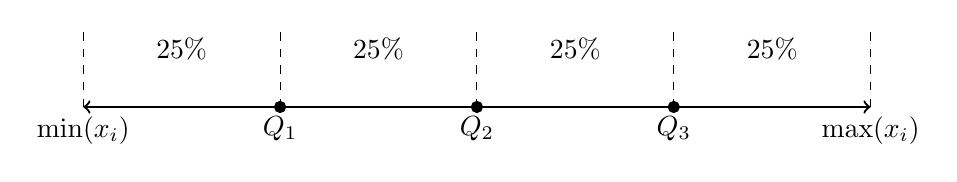
\begin{tikzpicture}[scale=1]
    % Draw a horizontal line with arrowheads at both ends
    \draw[<->, thick] (0,0) -- (10,0);

    % Label the endpoints of the line
    % 1) Mark and label min(x_i) at x=0
    \draw[dashed] (0,0) -- (0,1);
    \node[below] at (0,0) {min$(x_i)$};

    % 2) Mark and label max(x_i) at x=10
    \draw[dashed] (10,0) -- (10,1);
    \node[below] at (10,0) {max$(x_i)$};

    % Mark the quartile positions (Q1=25%, Q2=50%, Q3=75%)
    \foreach \x/\label in {2.5/Q_1, 5/Q_2, 7.5/Q_3} {
        % Place a small filled circle at each quartile
        \draw[fill=black] (\x,0) circle (2pt);
        % Draw a dashed vertical line for visual emphasis
        \draw[dashed] (\x,0) -- (\x,1);
        % Label the quartile below the dashed line
        \node[below] at (\x,0) {$\label$};
    }

    % Insert 25% labels in the middle of each segment
    % Segment 1: min to Q1
    \node[below] at (1.25,1) {25\%};
    % Segment 2: Q1 to Q2
    \node[below] at (3.75,1) {25\%};
    % Segment 3: Q2 to Q3
    \node[below] at (6.25,1) {25\%};
    % Segment 4: Q3 to max
    \node[below] at (8.75,1) {25\%};
\end{tikzpicture}
\end{frame}

\begin{frame}
\frametitle{Quartiles Example: Income Distribution}

Assume we have income data from a randomly selected sample. Below are the computed quartiles:

\vspace{1em}

{\centering
\begin{tabular}{|l|c|p{6cm}|}
\hline
\textbf{Quartile} & \textbf{Value} & \textbf{Interpretation} \\
\hline
\(\mathbf{Q_1}\)      & \$30{,}000 & 25\% of individuals earn \(\le\) \$30{,}000. \\
\(\mathbf{Q_2}\) (Median) & \$45{,}000 & 50\% of individuals earn \(\le\) \$45{,}000. \\
\(\mathbf{Q_3}\)      & \$82{,}000 & 75\% of individuals earn \(\le\) \$82{,}000. \\
\hline
\end{tabular}
\par
}
\vspace{1em} \pause % <-----|
\textbf{Note:} 
\begin{itemize}
    \item If someone earns \$84{,}100, they are \textbf{above} \(Q_3\) (or ``\emph{in} the third quartile"), meaning they earn more than 75\% of the sample.
    \item If someone earns \$23{,}500, they are \textbf{below} \(Q_1\) (or ``\emph{below} the first quartile"), meaning they earn less than 75\% of the sample (or ``are in the lowest 25\%"). 
\end{itemize}


\end{frame}


\begin{frame}
\frametitle{Deciles and Percentiles Example: Income Distribution}
\begin{itemize}
    \item \textbf{Deciles:} Divide the data into ten equal parts.
    \begin{itemize}
        \item \textbf{Ninth Decile Example:}
            \begin{itemize}
                \item 9th Decile = \$150,000: 90\% of individuals earn less than or equal to \$150,000.
            \end{itemize}
    \end{itemize}
    \item \textbf{Percentiles:} Divide the data into one hundred equal parts.
    \begin{itemize}
        \item \textbf{Ninety-Fifth Percentile Example:}
            \begin{itemize}
                \item 95th Percentile = \$400,000: 99\% of individuals earn less than or equal to \$400,000.
            \end{itemize}
    \end{itemize}
    \item \textbf{Interpretation:}
    \begin{itemize}
        \item Being at the 9th decile means you earn more than 90\% of the population.
        \item Being at the 99th percentile means you earn more than 99\% of the population.
    \end{itemize}
\end{itemize}
\end{frame}

\section{Measures of Dispersion}
\transitionslide{Measures of Dispersion}

\begin{frame}
\frametitle{Introduction to Measures of Dispersion}
\begin{itemize}
    \item \textbf{Definition:} Measures of dispersion describe a variable's the spread or variability. 
    \item \textbf{Purpose:} While measures of central tendency (like the mean or median) tell us about the center of the data, measures of dispersion help us understand the distribution's spread and how much individual data points deviate from the center.
\end{itemize}
\end{frame}


\begin{frame}{Comparing Two Discrete Distributions with the Same Mean}
\centering
\begin{minipage}{0.45\textwidth}
\centering
\textbf{Distribution 1: Wider Spread}\\
\begin{tikzpicture}[scale=0.9]
\begin{axis}[
    ybar,
    bar width=6pt,
    ymin=0,ymax=0.35,
    xmin=0.5,xmax=7.5,
    grid=major,
    width=\textwidth,
    height=5cm,
    xlabel={Value},
    ylabel={Relative Freq.},
    xtick={1,2,3,4,5,6,7},
]
  % Import table and plot
  \addplot table[x=x,y=y,col sep=comma] {dist1.csv};
\end{axis}
\end{tikzpicture}
\end{minipage}
\hfill
\begin{minipage}{0.45\textwidth}
\centering
\textbf{Distribution 2: Narrower Spread}\\
\begin{tikzpicture}[scale=0.9]
\begin{axis}[
    ybar,
    bar width=6pt,
    ymin=0,ymax=0.55,
    xmin=0.5,xmax=7.5,
    grid=major,
    width=\textwidth,
    height=5cm,
    xlabel={Value},
    ylabel={Relative Freq.},
    xtick={1,2,3,4,5,6,7},
]
  \addplot table[x=x,y=y,col sep=comma] {dist2.csv};
\end{axis}
\end{tikzpicture}
\end{minipage}
\end{frame}


\begin{frame}
\frametitle{Introduction to Measures of Dispersion}
\begin{itemize}
    \item \textbf{Range:} The difference between the maximum and minimum values.
    \begin{equation*}
        \text{Range} = \max \{x_i\} - \min \{x_i \}
    \end{equation*}
    \item \textbf{Interquartile Range (IQR):} The range between the first and third quartiles, highlighting the spread of the middle 50\% of the data.
    \begin{equation*}
        \text{IQR} = Q_3 - Q_1
    \end{equation*}
\end{itemize}
\end{frame}


\begin{frame}
\frametitle{Introduction to Measures of Dispersion}
\begin{itemize}
    \item \textbf{Variance:} The average of the squared deviations from the mean.
    \item \textbf{Standard Deviation:} The square root of the variance; representing the average deviation from the mean.
    \item \textbf{Mean Absolute Deviation:} The average of the absolute deviations from the mean
        \begin{equation*}
        \text{MAD} = \frac{\sum_{i=1}^N |x_i - \bar{x}|}{N}
    \end{equation*}
    \begin{itemize}
        \item \textbf{Note:} While the MAD can be a useful statistic to describe the variation in the data, we almost always focus on the Standard Deviation instead because of its useful properties for inference. 
    \end{itemize}
\end{itemize}
\end{frame}


\begin{frame}{Intuition for Squaring in Variance}
    \textbf{Distance Between Two Points in 2D}\\[6pt]
    The Euclidean distance between two points \( (x_i, y_i) \) and \( (\mu_x, \mu_y) \) is given by:
    \[
        d = \sqrt{(x_i - \mu_x)^2 + (y_i - \mu_y)^2}.
    \]
    
    \textbf{Why Squaring?}
    \begin{itemize}
        \item Squaring ensures all differences are positive, preventing cancellations.
        \item It naturally arises from the \textbf{Pythagorean theorem}, which measures true distance.
        \item Variance follows the same principle: it measures spread using squared differences from the mean.
        \item The standard deviation (square root of variance) gives a measure in the original units, just like distance.
    \end{itemize}
    
\end{frame}







\begin{frame}
\frametitle{Population vs. Sample Variance}

\begin{minipage}{0.48\textwidth}
\centering
\textbf{Population Variance}
\begin{itemize}
    \item Denoted by: $\sigma^2$
    \item Formula:
    \begin{equation*}
    \sigma^2 = \frac{1}{N} \sum_{i=1}^{N} (x_i - \mu)^2
    \end{equation*}
    \item Where:
    \begin{itemize}
        \item $N$ is the size of the population.
        \item $x_i$ is each individual value in the population.
        \item $\mu$ is the population mean.
    \end{itemize}
\end{itemize}
\end{minipage}
\hfill
\begin{minipage}{0.48\textwidth}
\centering
\vspace{-1em}
\textbf{Sample Variance}
\begin{itemize}
    \item Denoted by: $s^2$
    \item Formula:
    \begin{equation*}
    s^2 = \frac{1}{n-1} \sum_{i=1}^{n} (x_i - \bar{x})^2
    \end{equation*}
    \item Where:
    \begin{itemize}
        \item $n$ is the size of the sample.
        \item $x_i$ is each individual value in the sample.
        \item $\bar{x}$ is the sample mean.
    \end{itemize}
\end{itemize}
\end{minipage}

\end{frame}

\begin{frame}
\frametitle{Population vs. Sample Standard Deviation}

\begin{minipage}{0.48\textwidth}
\centering
\textbf{Population Standard Deviation}
\begin{itemize}
    \item Denoted by: $\sigma$
    \item Formula:
    \begin{equation*}
    \sigma = \sqrt{\frac{1}{N} \sum_{i=1}^{N} (x_i - \mu)^2}
    \end{equation*}
    \item Measures the average distance of each data point from the population mean $\mu$.
\end{itemize}
\end{minipage}
\hfill
\begin{minipage}{0.48\textwidth}
\centering
\textbf{Sample Standard Deviation}
\begin{itemize}
    \item Denoted by: $s$
    \item Formula:
    \begin{equation*}
    s = \sqrt{\frac{1}{n-1} \sum_{i=1}^{n} (x_i - \bar{x})^2}
    \end{equation*}
    \item Measures the average distance of each data point from the sample mean $\bar{x}$.
\end{itemize}
\end{minipage}
\end{frame}

\begin{frame}
\frametitle{Variance vs. Standard Deviation}
 \textbf{Why is Standard Deviation More Useful than Variance?}
    \begin{itemize}
        \item \textbf{Interpretability:} Standard deviation is in the same units as the original data, making it easier to interpret.
        \item \textbf{Comparison:} It allows for easier comparison between different datasets or distributions.
        \item \textbf{Practicality:} Many statistical methods and models use standard deviation rather than variance for these reasons.
    \end{itemize}
\end{frame}

\begin{frame}{Why the $N-1$ in the Sample Variance?}
\begin{itemize}
      \item \textbf{Correcting for Bias:}
    \begin{itemize}
        \item To correct for this bias, we divide by \( n-1 \) instead of \( n \).
        \item This adjustment, known as \textbf{Bessel's correction}, increases the variance slightly, providing an unbiased estimate of the population variance.
        \item By dividing by \( n-1 \), we account for the fact that the sample mean \(\bar{x}\) is an estimate and not the true population mean \(\mu\).
    \end{itemize}
    \vspace{1em}
    \item \textbf{Degrees of Freedom:}
    \begin{itemize}
        \item The use of \( n-1 \) reflects the concept of \textbf{degrees of freedom}, which represents the number of values in the final calculation that are free to vary.
        \item Since one degree of freedom is "lost" by using the sample mean, only \( n-1 \) independent pieces of information remain.
    \end{itemize}
\end{itemize}
\end{frame}


\begin{frame}
\frametitle{Coefficient of Variation (CV)}

\begin{minipage}{0.48\textwidth}
\centering
\begin{itemize}
    \item \textbf{Definition:} The Coefficient of Variation (CV) is defined as the ratio of the standard deviation (\(\sigma\)) to the mean (\(\mu\)):
    \[
    \text{CV} = \frac{\sigma}{\mu}
    \]
    \item Often expressed as a percentage:
    \[
    \text{CV} = \frac{\sigma}{\mu} \times 100\%
    \]
\end{itemize}
\end{minipage}
\hfill
\begin{minipage}{0.48\textwidth}
\centering
\begin{itemize}
    \item \textbf{Relative Measure:} CV provides a standardized measure of dispersion relative to the mean, allowing comparison between datasets with different units or scales.
    \item \textbf{Interpretation:} A higher CV indicates greater relative variability, while a lower CV suggests more consistency around the mean.
\end{itemize}
\end{minipage}

\end{frame}


\begin{frame}
\frametitle{Usefulness of the Interquartile Range (IQR)}

\begin{itemize}
    \item \textbf{Definition:} The Interquartile Range (IQR) is the difference between the third quartile (\(Q_3\)) and the first quartile (\(Q_1\)):
    \[
    \text{IQR} = Q_3 - Q_1
    \]
    \item \textbf{Key Benefits:}
    \begin{itemize}
        \item \textbf{Robustness:} IQR is not affected by outliers or extreme values, making it a robust measure of spread.
        \item \textbf{Focus on Middle 50\%:} IQR provides insight into the spread of the central 50\% of the data, highlighting the range within which the bulk of the data lies.
        \item \textbf{Comparison of Distributions:} IQR allows for easy comparison of variability between different datasets or distributions.
        \item \textbf{Identifying Outliers:} IQR is used to identify outliers; values that fall below \(Q_1 - 1.5 \times \text{IQR}\) or above \(Q_3 + 1.5 \times \text{IQR}\) are often considered outliers.
    \end{itemize}
\end{itemize}

\end{frame}


\end{document}